\documentclass[a4paper,11pt]{article}
\usepackage[francais]{babel}
\usepackage[utf8]{inputenc}
\usepackage[T1]{fontenc}
\usepackage{graphicx}
\usepackage{geometry}
\usepackage{amsmath}
\usepackage{float}
\usepackage{listings}
\usepackage{xcolor}
\usepackage{hyperref}

\setcounter{secnumdepth}{0}
\hypersetup{colorlinks=true, linkcolor=black}
\geometry{margin=1in}

\begin{document}

\selectlanguage{french}

\begin{titlepage}
    \begin{center}
        % Logo de l'école en en-tête
        
\includegraphics[width=5cm]{./img/uqac.png}\\[1cm]
        
        % Titre principal
        \vspace*{1cm} % Ajuster pour centrer verticalement
        {\Huge \textbf{Interaction Humain-Robot : Devoir 2}\\[0.5cm]}

        % Image de couverture (centrée en dessous du logo)
        \vspace*{1cm}
        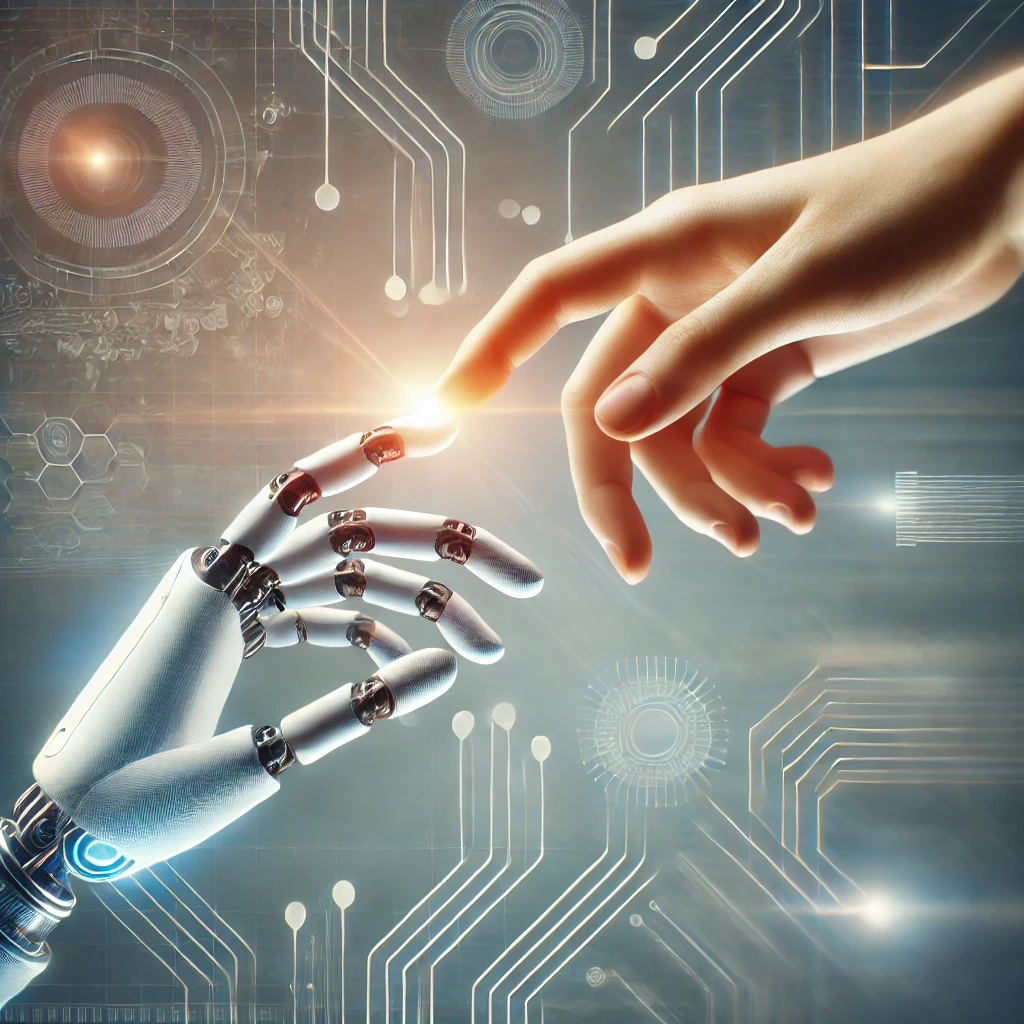
\includegraphics[width=0.7\textwidth]{./img/image_IHR.png}\\[1cm]

        
        
        % Informations des auteurs
        \vspace{2cm}
        {\LARGE Constance ALOYAU, Erwan MAWART, Benjamin PELLIEUX}
        
        \vspace{0.5cm}
        {\large PELB28120100, MAWE14050200, ALOC25530200}
        
        % Date
        \vspace{2cm}
        {\Large \today}
        
        \vfill
    \end{center}
\end{titlepage}

\tableofcontents
\newpage

\section*{Introduction}
    % à refaire...
    Les vibrations dans un mécanisme robotique, lorsqu’il est manipulé par un opérateur humain, peuvent affecter significativement la qualité et la précision de la tâche réalisée. Nous étudions l'impact perceptuel de ces vibrations lorsqu’un opérateur applique une force à l’aide d’une poignée sur un capteur de force fixé à un robot à un degré de liberté...

\section{Énoncé 1 : Conception du modèle du mécanisme}
\subsection{Question 1.1}
On note les variables d'états sont $x_{1}$, $x_{2}$, $v_{1}$ et $v_{2}$. En effet, une vitesse est la dérivée d'une position, d'où :
\[
    \begin{pmatrix}
        x_{1}\\
        x_{2}\\
        v_{1}\\
        v_{2}
    \end{pmatrix}
    =
    \begin{pmatrix}
        x_{1}\\
        x_{2}\\
        \dot{x_{1}}\\
        \dot{x_{2}}
    \end{pmatrix}
\]


Ainsi, on déduit les deux équations suivantes.
\[
    \begin{cases}
        m_{R}\ddot{x_{1}} = F - K_{B}x_{1} + K_{B}x_{2} - C_{B}\dot{x_{1}} + C_{B}\dot{x_{2}} \\
        M_{R}\ddot{x_{2}} = K_{B}x_{1} - K_{B}x_{2} + C_{B}\dot{x_{1}} - C_{B}\dot{x_{2}} - C_{R}\dot{x_{2}} \\
    \end{cases}
\]
\[
    \Leftrightarrow
    \begin{cases}
        \ddot{x_{1}} = \frac{F - K_{B}x_{1} + K_{B}x_{2} - C_{B}\dot{x_{1}} + C_{B}\dot{x_{2}}}{m_{R}} \\
        \ddot{x_{2}} = \frac{K_{B}x_{1} - K_{B}x_{2} + C_{B}\dot{x_{1}} - C_{B}\dot{x_{2}} - C_{R}\dot{x_{2}}}{M_{R}}
    \end{cases}
\]


Les variables d'état se constitue de deux équations matricielles : $\dot{X}=AX+BU$ et $Y=CX+DU$, où $A$, $B$, $C$ et $D$ sont à déterminer.
\[
    \dot{X}=AX+BU
    \Leftrightarrow
    \begin{bmatrix}
        \dot{x_{1}}\\
        \dot{x_{2}}\\
        \ddot{x_{1}}\\
        \ddot{x_{2}}
    \end{bmatrix}
    =
    \begin{bmatrix}
        0 & 0 & 1 & 0\\
        0 & 0 & 0 & 1\\
        \frac{-K_{B}}{m_{R}} & \frac{K_{B}}{m_{R}} & \frac{-C_{B}}{m_{R}} & \frac{C_{B}}{m_{R}}\\
        \frac{K_{B}}{M_{R}} & \frac{-K_{B}}{M_{R}} & \frac{C_{B}}{M_{R}} & \frac{-(C_{B}+C_{R})}{M_{R}}\\
    \end{bmatrix}
    \begin{bmatrix}
        x_{1}\\
        x_{2}\\
        \dot{x_{1}}\\
        \dot{x_{2}}
    \end{bmatrix}
    +
    \begin{bmatrix}
        0 & 0 & 0 & 0\\
        0 & 0 & 0 & 0\\
        0 & 0 & \frac{1}{m_{R}} & 0\\
        0 & 0 & 0 & 0\\
    \end{bmatrix}
    \begin{bmatrix}
        0\\
        0\\
        F\\
        0
    \end{bmatrix}\\
\]

\[
    Y=CX+DU
    \Leftrightarrow
    Y=CX
    \Leftrightarrow
    \begin{bmatrix}
        0\\
        x_{2}\\
        0\\
        \dot{x_{2}}
    \end{bmatrix}
    =
    \begin{bmatrix}
        0 & 0 & 0 & 0\\
        0 & 1 & 0 & 0\\
        0 & 0 & 0 & 0\\
        0 & 0 & 0 & 1\\
    \end{bmatrix}
    \begin{bmatrix}
        x_{1}\\
        x_{2}\\
        \dot{x_{1}}\\
        \dot{x_{2}}
    \end{bmatrix}\\
\]


\subsection{Question 1.2}
\begin{figure}[h!]
    \centering
    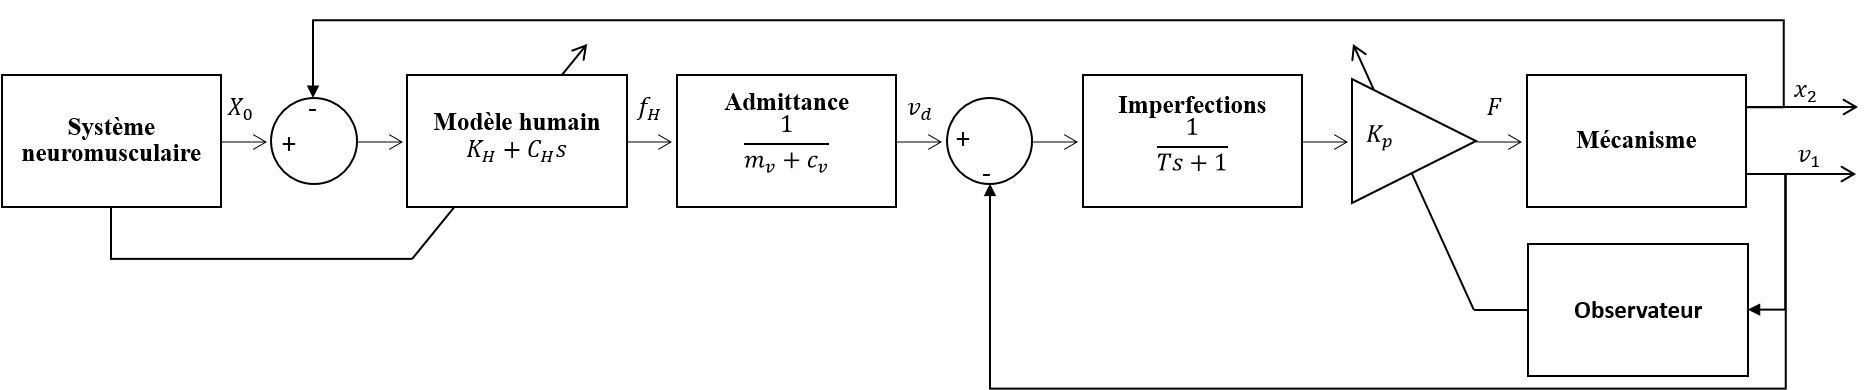
\includegraphics[width=16cm]{./img/SchemaBlocAvecObs.png}
    \caption{Schéma bloc du système avec observateur\label{fig:SchemaBlocAvecObs}}
\end{figure}

Un observateur est ajouté pour ajuster dynamiquement le gain correcteur $K_{p}$, qui est mis à jour selon la formule suivante :

\[
K_{p}(n+1) = K_{p}(n) \cdot \eta
\]

Où \eta =
\begin{cases}
    \eta_{\text{min}} & \text{si } \eta' \leq \eta_{\text{min}} \\
    \eta' & \text{si } \eta' > \eta_{\text{min}}
\end{cases}
\hspace{.5cm}, \hspace{.5cm} \eta' =
\begin{cases}
    1 & \text{si } V \geq V_{\text{min}} \\
    0 & \text{si } V \geq V_{\text{max}} \\
    \frac{V_{\text{max}} - V}{V_{\text{max}} - V_{\text{min}}} & \text{sinon}
\end{cases}

Et $V =$
\begin{cases}
    \lambda \sum_{i=1}^{q-1} \frac{\left| y_{1,i+1} - y_{1,i} \right|}{t_{1,i+1} - t_{1,i}} & \text{si } q \geq 2 \\
    0 & \text{si } q < 2
\end{cases}

Avec $\eta_{\text{min}}$ est une valeur définie proche de 0, $V_{\text{min}} = \frac{\lambda}{2}$, $V_{\text{max}} = V_{\text{min}} + \lambda$, $\lambda$ est un coefficient d’amplitude, $q$ représente le nombre d’extremums présents dans le signal, $y$ est l’amplitude du signal correspondant à l'${i}^{\text{ème}}$ extremum, et $t$ le temps correspondant.


\subsection{Question 1.3}
On a : 
$Den(s)=M_R T m_R^2 v \cdot s^6 + (M_R m_R^2 v + C_B T m_R^2 v + C_R T m_R^2 v + C_B M_R T m_R v + M_R T c m_R v) \cdot s^5 + (C_B m_R^2 v + C_R m_R^2 v + K_B T m_R^2 v + C_B M_R m_R v + K_p M_R m_R v + M_R c m_R v + C_B M_R T c v + C_B C_R T m_R v + K_B M_R T m_R v + C_B T c m_R v + C_R T c m_R v) \cdot s^4 + (K_B m_R^2 v + C_B M_R c v + C_B C_R m_R v + C_B K_p m_R v + K_p M_R c v + C_R K_p m_R v + K_B M_R m_R v + C_B c m_R v + C_R c m_R v + C_B C_R T c v + K_B M_R T c v + C_R K T m_R v + K_B T c m_R v) \cdot s^3 + (C_B C_R c v + C_B K_p c v + C_R K_p c v + K_B M_R c v + C_R K m_R v + K K_p m_R v + K c m_R v + C_R K T c v) \cdot s^2 + (C_B K_h K_p + C_R K c v + K K_p c v) \cdot s + K_B K_h K_p$
\\

\begin{center}
    \begin{tabular}{|c|c c c c|}
        \hline
        s^n & a_n & a_{n-2} & a_{n-4} & ...\\
        \hline
        s^{n-1} & a_{n-1} & a_{n-3} & a_{n-5} & ...\\
        \hline
        s^{n-2} & b_{n-1} & b_{n-3} & b_{n-5} & ...\\
        \hline
        s^{n-3} & c_{n-1} & c_{n-3} & c_{n-5} & ...\\
        \hline
        . & . & . & . & .\\
        . & . & . & . & .\\
        . & . & . & . & .\\
        \hline
        s^0 & h_{n-1} & h_{n-3} & h_{n-5} & ...\\
        \hline
    \end{tabular}
\end{center}

Où $b_{n-1}=\frac{-1}{a_{n-1}}$
\begin{vmatrix}
    a_n & a_{n-2} \\
    a_{n-1} & a_{n-3} \\
\end{vmatrix}
$=\frac{a_{n-1} a_{n-2} - a_n a_{n-3}}{a_{n-1}}$,
$b_{n-3}=\frac{-1}{a_{n-1}}$
\begin{vmatrix}
    a_n & a_{n-4} \\
    a_{n-1} & a_{n-5} \\
\end{vmatrix}
, etc.\\

Et $c_{n-1}=\frac{-1}{b_{n-1}}$
\begin{vmatrix}
    a_{n-1} & a_{n-3} \\
    b_{n-1} & b_{n-3} \\
\end{vmatrix}
, $c_{n-3}=\frac{-1}{b_{n-1}}$
\begin{vmatrix}
    a_{n-1} & a_{n-5} \\
    b_{n-1} & b_{n-5} \\
\end{vmatrix}
, etc.\\



\section{Énoncé 2 : Simulation}
\subsection{Question 2.1}

\subsection{Question 2.2}

\subsection{Question 2.3}

\section{Annexe}
\subsection{Lien vers le Dépôt GitHub}
\url{https://github.com/BlueWan14/Cours_IHR/tree/main/Devoir_2}

\end{document}
